\chapter{Étude Conceptuel et architectural}
\label{sec:conception}

\begin{fquote}Dans ce chapitre nous allons nous concentrer sur l’aspect conceptuel et architectural de la solution à mettre en place. Cette étude conceptuelle est basée sur l’élaboration et l’analyse des différents schémas et diagrammes de classes.
 \end{fquote}

\clearpage

\section{Introduction}

L'organisation de l'entreprise cliente repose sur le maillage de trois divisions : la Mode (Fashion), les Parfums Beauté (fragrance and beauty) et l'Horlogerie Joaillerie (Watches And Fine Jewelry). La plate-forme Hybris est potentiellement utilisée pour les 3 divisions.

\medskip

Pour ce qui concerne la solution PIM, elle est principalement implémentée pour les deux divisions de Mode et d'Horlogerie Joaillerie. Pour cela, une partie de la modélisation de cette solution est partagée entre les deux solutions, et ce pour remédier à la répétition et mettre en valeur les éléments communs entre les deux divisions.

\medskip

Le présent projet porte sur la solution PIM de la division Horlogerie Joaillerie. Pour des raisons de lisibilité, on préfixera dans le reste de ce chapitre les entités et notions propre à cette division avec le préfixe WFJ (Watches and Fine Jewelry) et pour les entités et notions communes entre les deux divisions avec le préfixe PIM.

\section{Modèle de données}
\subsection{Catalogue et versions}

Hybris est une solution logicielle centrée sur le principe de catalogue de produits afin de gérer les données des produits, connu aussi sous le nom de PCM (Product Content Management). Ce catalogue est composé de plusieurs versions et regroupe l'ensemble des produits avec leurs données relatives (voir la figure \ref{fig:classes-catalogue}).

\begin{figure}[ht]
  \centering
  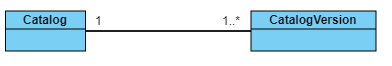
\includegraphics{catalog-classes.png}
  \caption{Aperçu du diagramme de classes du catalogue et ses versions.}
  \label{fig:classes-catalogue}
\end{figure}
\FloatBarrier


\medskip

Notre solution PIM s'appuie sur ce principe. Par la suite, on utilise les deux versions de catalogue \textbf{Staged} et \textbf{Online} pour distinguer les données en cours d'enrichissement des données publiées (utilisables pour être exportées).

\medskip

La réplication des données d'une version du catalogue à l'autre est effectué à partir d'un traitement de \textbf{Synchronisation} natif à hybris, qui est à son tour possible à travers le principe du \textbf{Catalog Aware} d'Hybris.

\medskip

Ce processus est un job d'Hybris qui sélectionne les produits et les autres éléments du système qui sont \textbf{Catalog Aware} de la version intermédiaire ou \textbf{Staged}, vérifie la présence de certaines règles (indiquant que l'élément est prêt à être mis en ligne ou publié) et crée (ou la met à jour s'il est déjà créé) une copie de l'élément avec la version En ligne ou \textbf{Online}.

\medskip

Le principe du \textbf{Catalog Aware} sert à indiquer les produits ou les entités devraient avoir deux copies dans le système, afin que les utilisateurs professionnels puissent apporter les modifications appropriées avants leurs publication. Ces éléments sont appelés \textbf{Catalog Aware} et entrent dans le processus de synchronisation. Or les autres éléments du systeme qui ne participent pas ou ne devraient pas participer au processus de synchronisation sont appelés \textbf{Catalog Unaware}.

\medskip

La figure \ref{fig:catalog} illustre le principe du catalogue et des versions de catalogue d'Hybris, implémenté dans la plate-forme PIM sous le nom de \textbf{WFJProductCatalog}:


\begin{figure}[ht]
  \centering
  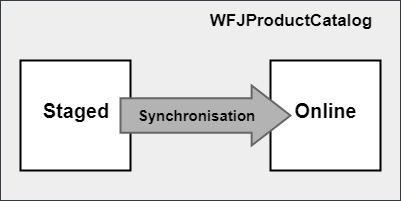
\includegraphics[width=10cm]{catalog.png}
  \caption{Le principe du catalogue des produits d'Hybris.}
  \label{fig:catalog}
\end{figure}
\FloatBarrier

On suit donc les règles de gestion suivantes pour adapter ce système aux besoins de notre solution PIM:

\medskip

\begin{itemize}
    \item[$\bullet$] L'import des données se fait sur la version Staged.
    \medskip
    \item[$\bullet$] L'enrichissement des données se fait sur la version Staged.
    \medskip
    \item[$\bullet$] Lorsqu'un produit est correctement enrichi, il est manuellement passé à l'état "approved". 
    \medskip
    \item[$\bullet$] L'export des données se fait à partir de la version Online.
    \medskip
    \item[$\bullet$] Le système de synchronisation recopie les données de la version Staged vers la version Online pour tous les produits qui sont à l'état "approved".
    \medskip
    \item[$\bullet$] Si un produit change d'état d'approbation sur la version Staged
    \smallskip
    
    \begin{itemize}
        \item Il n'est plus synchronisé sur la version Online.
            \smallskip

        \item Mais il reste présent sur la version Online (avec les données de la dernière synchronisation).
    \end{itemize}
\end{itemize}

On met en place un traitement (cronjob) de synchronisation, basé sur le fonctionnement natif hybris, permettant de répliquer les données du catalogue (produits avec leurs attributs, catégories, etc.) de la version \textbf{Staged} vers la version \textbf{Online}. Les entités qui sont synchronisées sont :

\begin{itemize}
        \item[$\bullet$] Produits (et toutes les déclinaisons)
        \smallskip
        \item[$\bullet$] Catégories (et toutes les déclinaisons)
        \smallskip
        \item[$\bullet$] Médias (et toutes les données associées)
\end{itemize}
\medskip

Les processus d'import, d'enrichissement et d'export se résument dans la figure \ref{fig:synchronisation} :
\begin{figure}[ht]
  \centering
  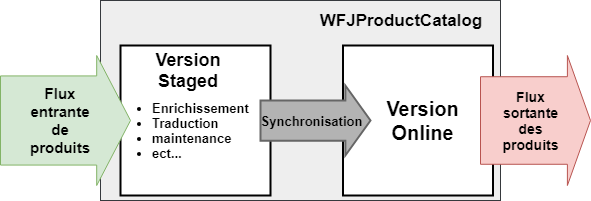
\includegraphics[width=14cm]{synchronization.png}
  \caption{Récapitulatif du processus de Synchronisation.}
  \label{fig:synchronisation}
\end{figure}
\FloatBarrier
\subsection{Les produits}

Tous les produits de la division Horlogerie Joaillerie ou WFJ (Watches And Fine Jewelry) sont gérés à partir de l'ERP central, nommé CERP et basé sur la solution technique Microsoft AX. Indépendamment de leurs typologies, les produits WFJ sont déclinés suivant 2 à 3 niveaux de variante : \textbf{Référence} (entité produit de base qui contient la plupart des attributs de base du produit) déclinées en \textbf{SKU} (variation du produit de base selon un certain attribut comme la taille ou la couleur) et éventuellement \textbf{Matricule} (pour les pièces numérotées).\\

Le schéma de la figure \ref{fig:herarchie_product} illustre cette hiérarchie des produits:

\begin{figure}[ht]
  \centering
  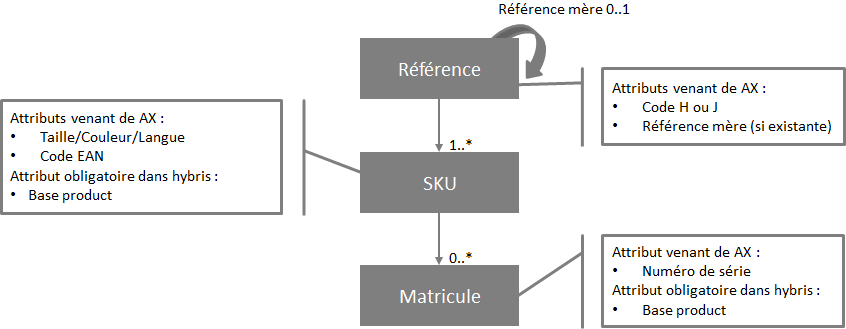
\includegraphics[width=15cm,height=5.6cm]{herarchie_product.png}
  \caption{Récapitulatif de l'abstraction du produit.}
  \label{fig:herarchie_product}
\end{figure}
\FloatBarrier


\subsubsection{Les Références ou les produits de base :}

La \textbf{Référence} est équivalente au \textbf{Product} dans le modèle de données natif d'Hybris. On définit donc la référence dans notre solution avec L'entité \textbf{WfjProduct}, en héritant de ce modèle.
\medskip

Chaque référence est unique et possède un code (unique) défini dans l'ERP est utilisé telquel dans le PIM.
\medskip
\begin{itemize}
    \item[$\bullet$] Dans AX, l'horlogerie et la joaillerie ont chacune une base de données distincte même si certaines données référentielles sont communes aux deux.
    \smallskip
    \item[$\bullet$] Les références de joaillerie ont un code commençant par un \textbf{J}.
    \smallskip
    \item[$\bullet$] Les références d'horlogerie ont un code commençant par un \textbf{H}
    \smallskip
    \item[$\bullet$] Une référence peut avoir une référence mère ; nommée masterProduct coté PIM.
    \smallskip
    \item[$\bullet$] Les références sont identifiables par leur \textbf{code} (\textbf{H} ou \textbf{J}), il s'agit de leur clé d'unicité.

\end{itemize}
\medskip

Pour définir les variations d'une certaine \textbf{Référence} on a introduit la notion de \textbf{Grille de Tailles}, modélisée par l'entité \textbf{WfjErpSizeGrid}. Cette entité est liée à la référence (WfjProduct) et porte les différents valeurs possibles de la \textbf{Taille} modélisée par l'entité \textbf{WfjErpSize} et représentant le paramètre du variation de cette référence.
\medskip

Cette notion de grille de taille et détournée pour représenter non seulement les variations de vraies tailles (S, M, X, XL, ...) mais aussi des variations de couleurs ou de langues (pour les catalogues imprimés).

\subsubsection{Les SKUs ou les variants du produit selon la taille :}
Le \textbf{SKU} est la variante de produit basée sur l'attribut de taille en fonction de la grille de la taille renseignée sur la \textbf{Référence}. Les \textbf{SKU}s sont présentés dans le PIM par l'entité \textbf{WfjSkuVariant}.
\bigskip
\begin{itemize}
    \item[$\bullet$] Un SKU est lié à une et une seule Référence via l'attribut \textit{"baseProduct"} et une référence peut avoir plusieurs SKU.
    \smallskip
    \item[$\bullet$] la notion de taille est légèrement détournée dans AX pour certains types de produits. En effet, certaines grilles "de taille" sont déclarées pour gérer des déclinaison de couleur ou de vraies tailles.
    \smallskip
    \item[$\bullet$] Les SKU sont identifiables par leur \textbf{code} de référence de rattachement et leur \textbf{taille} (ou leur position dans leur grille de taille), les deux forment la clé d'unicité.
\end{itemize}

\subsubsection{Les Matricules ou les pièces numérotées :}

Les \textbf{Matricules} sont les produits réels dans le cas de pièce numérotées. Chaque matricule représente une version unique d'un SKU et possède donc un numéro de série unique (généré par AX). Les Matricules sont présentés dans le PIM par l'entité \textbf{WfjSerialNumberVariant}.
\medskip

\begin{itemize}
    \item[$\bullet$] Un matricule est lié à un et un seul SKU via l'attribut \textit{"baseProduct"}. Un SKU peut avoir plusieurs matricules.
\medskip
    \item[$\bullet$] Les matricules sont identifiables par (autrement dit, la clé d'unicité est le triplet) :
\medskip
    \begin{itemize}
    \smallskip
        \item Leur \textbf{code} de Référence de rattachement.
        \smallskip
        \item Leur \textbf{taille} (ou leur position dans leur grille de taille).
        \smallskip
        \item Leur \textbf{numéro de série}.
    \end{itemize}
\end{itemize}
\medskip

Le diagramme de classes de la figure \ref{fig:classes-diagram} présente les différentes classes utilisés pour représenter le modèle du produit. Il met en évidence avec trois couleurs les classes qui sont natives à Hybris (en bleu) et les classes qui sont communes avec les autres divisions où est implémenté le PIM (en orange et préfixées par PIM) et celles conçues spécifiquement pour les produits de la division WFJ (en rose et préfixées par WFJ).

\begin{figure}[ht]
  \centering
  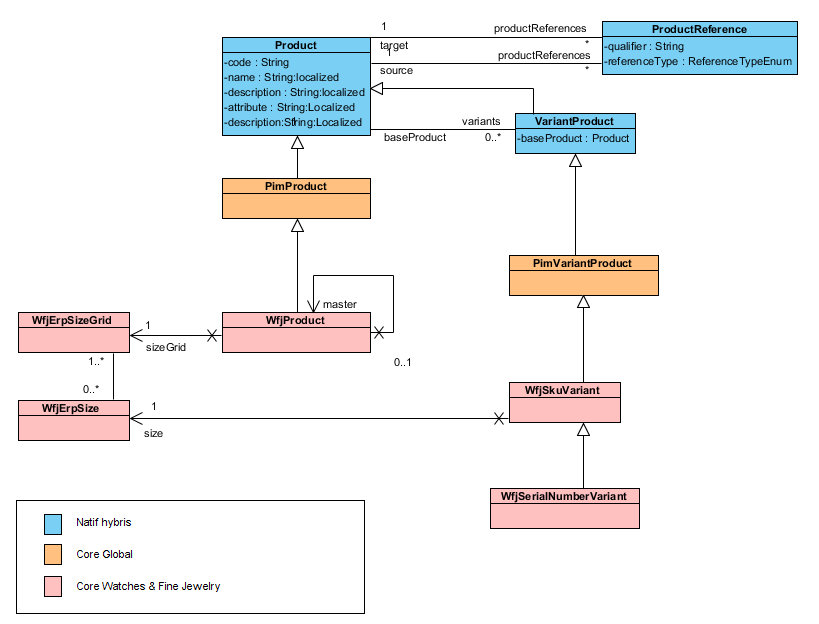
\includegraphics[width=17cm]{classes-diagram.png}
  \caption{Diagramme de classes des produits.}
  \label{fig:classes-diagram}
\end{figure}
\FloatBarrier
\medskip

Comme le montre la figure \ref{fig:classes-diagram},les différentes entités présentées dans ce diagramme sont comme suit:

\medskip

\begin{itemize}
    \item[$\bullet$] \textbf{WfjProduct}, hérite de \textbf{PimProduct} qui hérite à son tour, de L'entité \textbf{Product} d'Hybris est constitue la \textbf{Référence} présenté précédement.
    \medskip
    \item[$\bullet$] \textbf{WfjProduct} peut avoir un master product du même type permettant de mettre en oeuvre des systèmes d'héritage des données, c'est à dire de déduire certaines informations d'une référence à partir de sa référence master.
    \medskip
    \item[$\bullet$] \textbf{ProductReference} permet d'établir un lien entre de produit en spécifiant le type de ce lien et les deux produits source et target.
    \medskip
    \item[$\bullet$] \textbf{WfjProduct} porte la notion de \textit{"SizeGrid"} (grille de déclinaisons de taille).
    \medskip
    \item[$\bullet$] \textbf{WfjErpSizeGrid} Les grilles de tailles proviennent d'AX. Le concept de grille de taille est étendu (détourné) pour pouvoir gérer des tailles mais aussi des langues ou des couleurs.
    \medskip
    \item[$\bullet$] \textbf{WfjSkuVariant}, represente le \textbf{SKU} introduit précédemment et hérite de PimVariantProduct qui, à son tour, hérite du VariantProduct du modèle natif d'Hybris, représentant des variations du produit en question comme par exemple au niveau de la taille (S, M, L, XL...) ou la couleur.
    \medskip
    \item[$\bullet$] \textbf{WfjErpSize}, La taille indique l'information liée à la grille des tailles de la référence.
    \begin{itemize}
        \smallskip
        \item Si la référence est liée à la grille des tailles "Taille", alors l'id sera une taille.
                \smallskip
        \item Si la référence est liée à la grille des tailles "Couleur", alors l'id sera une couleur et la taille du produit sera unique.
    \end{itemize}
    \medskip
     \item[$\bullet$] \textbf{WfjSerialNumber}, represente le \textbf{Matricule} introduit précédemment et hérite de \textbf{WfjSkuVariant}, il représente les produits réels dans le cas de pièce numérotées. Chaque matricule représente une version unique d'un SKU et possède donc un numéro de série unique (généré par AX).
\end{itemize}

On suit ainsi les règles de gestion suivantes pour les réferences et les grilles de taille :

\begin{itemize}
    \item[$\bullet$] On affecte toujours une et une seule grille de taille à une référence (WfjProduct) et une référence doit toujours posséder une grille de taille (WfjErpSizeGrid).
    \medskip
    \item[$\bullet$] La grille de taille unique \textit{"UNI"} permet de gérer les cas où il n'y a pas de variation de la référence.

    \medskip
    \item[$\bullet$] Les grilles de tailles sont importées dans le PIM à partir du flux AX.
\end{itemize}

\subsection{Les catégories}

La plate-forme PIM permet de regrouper les produits dans des catégories. Ces catégories peuvent être structurées en arborescences et on identifie trois grandes typologies de catégories (voir la figure \ref{fig:classes-caegories}) :

\medskip

\begin{itemize}
        \item[$\bullet$] \textbf{ERP Category} : catégories permettant de représenter l'arborescence de l'ERP. Ces catégories et leurs liaisons sont répliquées à partir de flux de données en provenance de l'ERP et ne sont pas suceptible d'être modifié dans le PIM.
        
\medskip

        \item[$\bullet$] \textbf{Communication Category} : catégories permettant de constituer l'arborescence principale de communication, autrement dit, de créer une autre arborescence à partir de celle de l'ERP pour le modifier et l'évoluer au besoin.
        
\medskip

        \item[$\bullet$] \textbf{Tags Category} : catégories moins structurées, permettant d'organiser les produits de manière plus libre et avec d'éventuelles redondances.
\end{itemize}

\begin{figure}[ht]
  \centering
  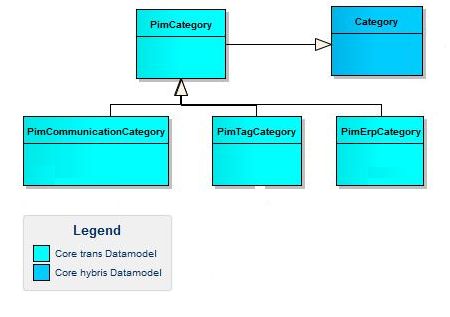
\includegraphics{categories.png}
  \caption{Diagramme de classe des catégories.}
  \label{fig:classes-caegories}
\end{figure}
\FloatBarrier

\subsection{Les medias}

Le DAM (Digital Asset Management) permet de gérer des Assets ; c'est à dire des ressources numériques (principalement des images, scan PDF et vidéos) visant à être présentées sur des canaux digitaux ou autres supports papiers \cite{wiki:dam}.

\medskip

\begin{itemize}
    \item[$\bullet$] Les Assets du \textbf{DAM} sont matérialisées à partir de l'entité native d'Hybris : \textbf{MediaContainer}.
    \smallskip
    \item[$\bullet$] Tout ou partie des \textbf{métadonnées} d'un Asset sont stockées dans des attributs du \textbf{MediaContainer} correspondant.
    \smallskip
    \item[$\bullet$] Les formats de déclinaison des Assets du DAM sont configurés en tant que \textbf{MediaFormat} hybris (entité native de formats des médias).
    \smallskip
    \item[$\bullet$] Les différentes déclinaisons, dans différents formats, d'un même Asset du DAM sont chacune matérialisées par un \textbf{Media} dans hybris. Chaque Media concerne un format donné.
    \medskip
    \item[$\bullet$] Tous les Medias sont regroupés au sein du \textbf{MediaContainer} représentant l'Asset.
\end{itemize}

Le diagramme de classes de la figure \ref{fig:classes-media} représente ces différents classes et leurs relations:

\begin{figure}[ht]
  \centering
  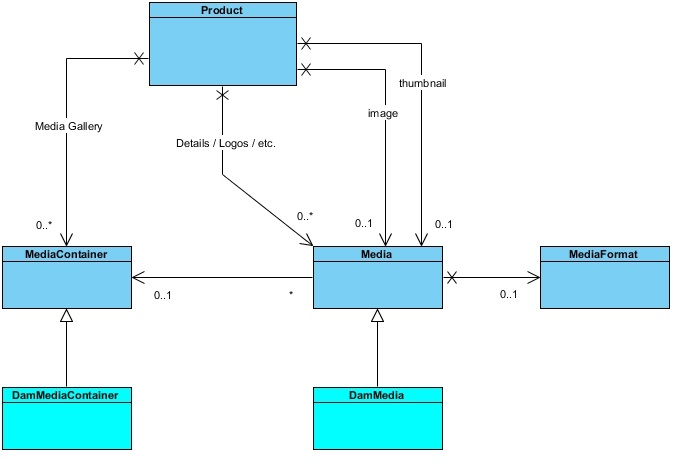
\includegraphics{media-classes.jpg}
  \caption{Diagramme de classe des médias.}
  \label{fig:classes-media}
\end{figure}
\FloatBarrier
\section{Le flux d'import}

Le socle d'import permet d'importer des données depuis des systèmes tiers qui sont l'ERP centrale et le DAM du client vers le PIM. Il permet, par exemple, d'importer des produits ou des données référentielles ou encore des prix de produits.

\medskip

Le socle d'import consomme des fichiers XML de données et plus précisément des fichiers au format CBL. En règle générale, les fichiers à importer dans le PIM sont mis à disposition par l'EAI Biztalk (qui prend donc en charge le transport des fichiers importés).

\medskip

Le socle d'import fonctionne suivant un principe dit de "hotFolder" ; c'est à dire que les fichiers déposés dans les dossiers d'entrée (Splitting ou In) sont automatiquement consommés et traités dès lors qu'ils respectent une règle de nommage prédéfinie.

\medskip

Le processus d'import comporte 3 principaux traitements comme le montre la figure \ref{fig:import} :

\begin{figure}[ht]
  \centering
  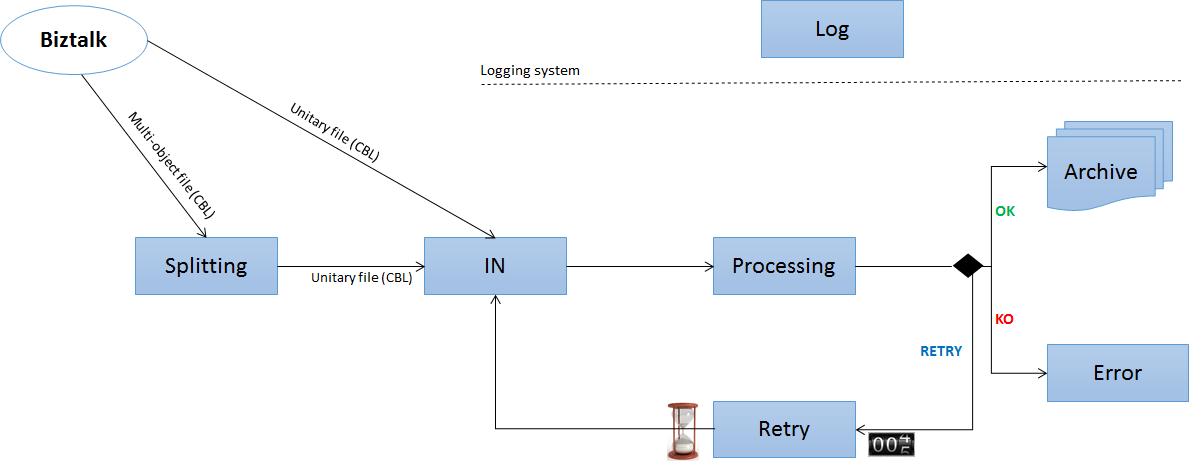
\includegraphics[width=17cm]{import.png}
  \caption{Processus d'import des produits.}
  \label{fig:import}
\end{figure}
\FloatBarrier

\begin{itemize}
    \item[$\bullet$] \textbf{Splitting :} gère le découpage d'un fichier XML au format CBL\footnote{Common Business Library : un format des fichiers XML utilisé dans l'ecommerce\cite{xcbl}} de collection d'objets en de multiples fichiers unitaires
    \smallskip
    \begin{itemize}
        \item L'opération de découpage n'est pas systématique. Pour la plupart des flux de données, Biztalk livre des fichiers unitaires qu'il dépose directement dans le dossier d'import.
    \end{itemize}
    \medskip
    \item[$\bullet$] \textbf{Import :} étape d'injection des données d'un fichier unitaire vers un objet dans le PIM.
    \medskip
    \item[$\bullet$] \textbf{Retry :} traitement de relances multiples de l'import de fichiers unitaires ayant rencontré une erreur lors de l'import.
\end{itemize}

Une operation de \textbf{logging} ou journalisation et mise en place tout au long du processus d'import pour garder la traçabilité des différentes étapes et donc d'identifier les sources des éventuelles erreurs.

\subsubsection{Traitement "splitting" :}

Le Traitement de \textbf{splitting} est illustré dans la figure \ref{fig:splitting1} :

\begin{figure}[ht]
  \centering
  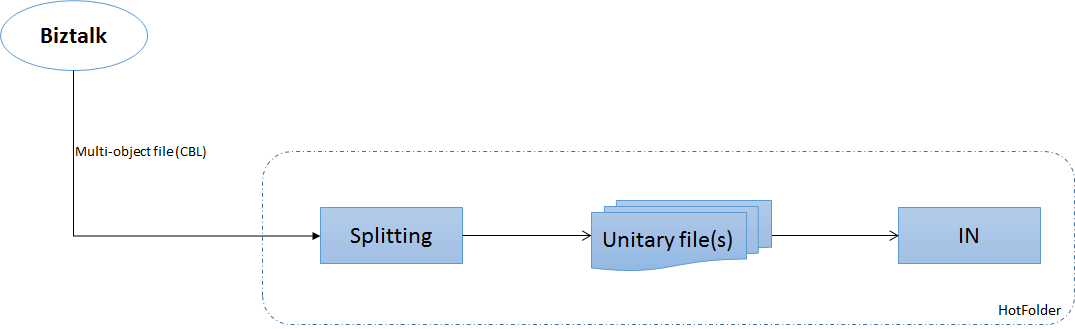
\includegraphics[width=17cm]{splitting1.png}
  \caption{Processus de splitting des fichiers xml.}
  \label{fig:splitting1}
\end{figure}
\FloatBarrier

Le traitement permet de découper des fichiers CBL contenant plusieurs objets de données (produits) en de multiples fichiers unitaires (contenant respectivement les données d'un seul produit) voir la figure \ref{fig:splitting}.
\medskip

\begin{figure}[ht]
  \centering
  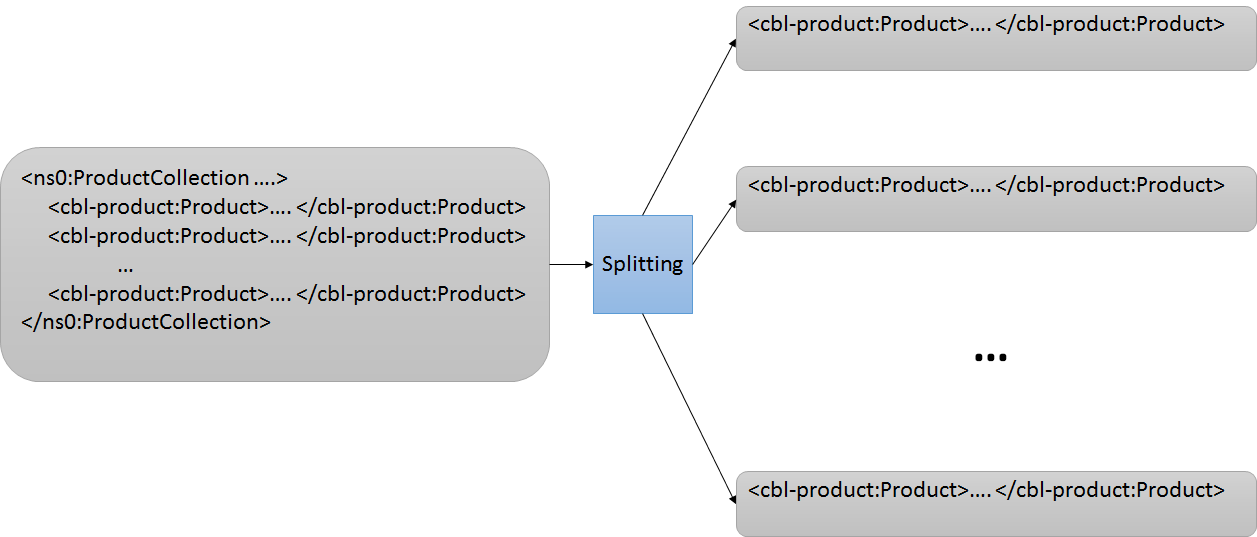
\includegraphics[width=17cm]{splitting.png}
  \caption{Splitting d'un fichier multiple vers des fichier unitaire.}
  \label{fig:splitting}
\end{figure}
\FloatBarrier

\begin{itemize}
    \item Le dossier d'entrée du traitement de découpage est le dossier "splitting".
    \medskip
    \item Le traitement est en mode "\textbf{hotFolder}".
    \medskip
    \item Le traitement lit le contenu du fichier initial (à découper) et génère à la volée (au fûr et à mesure) les fichiers unitaires.
    \medskip
    \item Chaque fichier généré est automatiquement déposé dans le dossier d'import.
    \medskip
    \item Les fichiers unitaires suivent une règle de nommage particulière et intégrant l'identifiant de l'objet qu'ils représentent
\end{itemize}

\subsubsection{Traitement "Import":}

Le traitement d'import d'un fichier de données commence par déplacer le fichier à importer dans un dossier de travail : \textit{Processing}. Certains contrôles (dépendant de l'entité de donnée importée) sont effectués lors de l'import.
\medskip

En fonction du bon déroulement de l'import et des contrôles, le fichier est déplacé dans l'un des dossiers suivants :

\begin{itemize}
\medskip
    \item \textbf{Archive :} si l'import est effectué avec succès
    \smallskip
    \item \textbf{Error :} si l'import à échoué
    \smallskip
    \item \textbf{Retry :} si l'on souhaite refaire de nouvelles tentatives d'import du même fichier unitaire.
\end{itemize}

\subsubsection{Traitement "Retry" :}

Le traitement de Retry permet de relancer l'import d'un fichier qui aurait rencontrée un erreur lors d'un import.

\medskip

Le traitement de Retry s'appuie sur 2 paramètres :
\begin{itemize}
\medskip
    \item Le délai d'attente avant un Retry
    \smallskip
    \item Le nombre de tentatives de Retry
\end{itemize}
\medskip
Le principe du traitement est :
\medskip
\begin{itemize}
    \item Après un import \textit{"normal"} avec erreur, le fichier importé est placé dans le dossier \textbf{Retry}.
    \smallskip
    \item Après le délai d'attente du retry, le fichier est de nouveau déplacé vers le dossier d'import ( \textbf{In}) ; et le système comptabilise la nouvelle tentative d'import.
    \smallskip
    \item L'opération est répétées tant que le fichier soulève une erreur (configurée pour le retry).
    \smallskip
    \item Si le nombre de tentative est atteint, après un nouvel import avec erreur, le fichier est finalement déplacé dans le dossier d'erreur (\textbf{error})
\end{itemize}
\clearpage
\section{Architecture Logiciel du projet}
Notre solution est basée sur la plate-forme SAP Hybris et suit donc son architecture logicielle présentée dans la figure \ref{fig:architecture}:

\begin{figure}[ht]
  \centering
  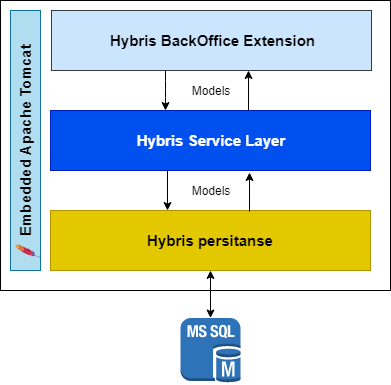
\includegraphics[height=9cm]{architecture.png}
  \caption{Architecture logiciel du projet.}
  \label{fig:architecture}
\end{figure}
\FloatBarrier


\begin{itemize}
    \item[$\bullet$] la plate-forme Hybris inclut un serveur \textbf{Apache Tomcat} constituant son serveur Http.
    \medskip
    \item[$\bullet$] \textbf{l'extension Backoffice d'hybris:} c'est une extension Hybris qui permet aux utilisateurs métier d'avoir accès aux différentes fonctionnalités d'administration du contenu que se soit le catalogue, les catégories ou les produits ainsi que les différentes entités et types du système.
    \begin{itemize}
    \smallskip
        \item l'extension backoffice est basée sur le framework web \textbf{ZK}.
        \smallskip
        \item cette extension permet aux développeurs de créer ou bien de personnaliser les composants Hybris selon leurs besoins.
    \end{itemize}
    \medskip
    \item[$\bullet$] \textbf{Le service Layer} de Hybris constituant la couche métier où il est implémenté la logique du business, il est constitué à sont tour d'un ensemble de couches de services et communique avec le backoffice et la couche de persistance à travers les \textbf{Models} (les entités de la logique métier).
    \medskip
    \item[$\bullet$] \textbf{La couche persistance} d'hybris est l'intermédiaire entre la base de données \textbf{MS SQL Server} est le Service Layer.
    
\end{itemize}

\section{Architecture physique du projet}

Cette partie présente l’architecture physique du projet, avec les différents serveurs utilisés. L’architecture de notre projet est composé de deux parties : interne et externe.

\medskip

La partie interne est l'architecture implémentée au niveau de SQLI Rabat, elle est essentiellement composée d'un seul serveur d'intégration INT (Integation) en plus du serveur SonarQube\footnote{\url{https://www.sonarqube.org/}} (un logiciel libre permettant de mesurer la qualité du code source en continu \cite{wiki:sonarqube}) pour l'analyse du qualitée de code. 

\medskip

La partie externe est celle implémentés dans l'environnement client et composée de trois serveurs: UAT pour le User Acceptence Testing, OAT pour l'Operational Acceptence Testing et PROD le serveur de production.
\medskip

La figure \ref{fig:architecture2} illustre cette répartition:

\begin{figure}[ht]
  \centering
  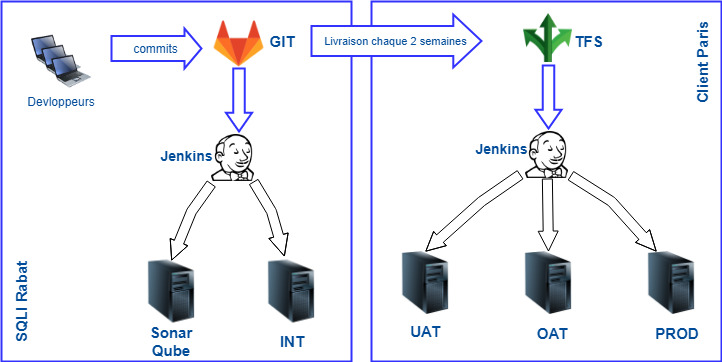
\includegraphics[width=17cm]{physique.png}
  \caption{Architecture physique du projet.}
  \label{fig:architecture2}
\end{figure}

Les équipes de développement font des commits sur le serveur GIT (Gitlab), en suite un serveur d’intégration continue Jenkins (PIC ou Plate-forme d'Intégration Continue) récupère les versions produites depuis le GIT pour faire un build automatique avec ANT (un outil d'automatisation des opérations de build ou compilation des applications JAVA \cite{wiki:ant}) et lance une analyse Sonar depuis le serveur SonarQube sur le code afin de garantir sa qualité.
\medskip

Après avoir fais les analyses Sonar le serveur vérifie que le nombre d'erreurs trouvé ne dépasse pas les limites prédéfinies selon le degré de gravité des erreurs et les quotas définis dans le serveur SonarQube et notifie les développeurs des résultats d'analyse, puis il fait le déploiement dans le serveur d’intégration (INT).
\medskip

Ce processus d'intégration continue se répète tous au longe du sprint qui dure deux semaine et se termine par le livraison d'une nouvelle version au client dans son système de contrôle des versions TFS (Team Foundation Server).
\medskip

Le client dispose de trois serveurs dont deux serveurs de test et un serveur de production:
\medskip

\begin{itemize}
    \item Le serveur UAT (User Acceptence Testing) sert à tester les livrables et s'assurer qu'ils correspondent aux attentes de l'utilisateur final.
\smallskip
\item Le serveur OAT (Operational Acceptence testing) est un serveur qui permet de déterminer si les livrables sont opérationnelles et près à intégrer l'environnement de production.
\smallskip
\item Après ces différents processus de test et dans chaque trois mois  une opération de mise en production (MEP) s'effectue  dans le serveur PROD pour qu'il soit disponible en ligne à l'utilisateur final.
\end{itemize}


\section{Conclusion}

Ce chapitre présente une vue conceptuelle de la solution à mettre en place. Il expose les différents diagrammes UML pour mieux comprendre les fonctionnalités offertes et pour mieux représenter la communication entre les différents objets du projet. Le chapitre suivant, présente la partie mise en œuvre de l’application.


